%%%%%%%%%%%%%%%%%%%%%%%%%%%%%%%%%%%%%%%%%%%%%%%%%%%
%
%  New template code for TAMU Theses and Dissertations starting Fall 2012.  
%  For more info about this template or the 
%  TAMU LaTeX User's Group, see http://www.howdy.me/.
%
%  Author: Wendy Lynn Turner 
%	 Version 1.0 
%  Last updated 8/5/2012
%
%%%%%%%%%%%%%%%%%%%%%%%%%%%%%%%%%%%%%%%%%%%%%%%%%%%
%%%%%%%%%%%%%%%%%%%%%%%%%%%%%%%%%%%%%%%%%%%%%%%%%%%%%%%%%%%%%%%%%%%%%%
%%                           SECTION III
%%%%%%%%%%%%%%%%%%%%%%%%%%%%%%%%%%%%%%%%%%%%%%%%%%%%%%%%%%%%%%%%%%%%%

\chapter{\uppercase{Related Work and State of Art}}

There are so many research scientists working in large oil \& gas companies and related service companies, but in such a mature industry, it is very difficult to find complete open source codes or complete sample data on Internet. The main reason should be Intellectual Property issue; In the last twenty years, the oil \& gas becomes the most profitable industry. As there is less unexplored area, how to find the valuable oilfield is the most important task for oil \& gas companies. With the intensifying competition, the exploration data became very expensive and every company either kept its technology secret or applied for patents to protect itself.    

In normal case of seismic data processing, most companies will both write their own algorithms and use commerical softwares such as MATLAB, Petrel from Schlumberger, Paradigm software suite etc. The previous ones are mostly used to verify and its own customized algorithms or models that could be optimized basing on requirement, on the other hand, commercial softwares are mainly used in imaging and interpretation stages. But most of them could only run on single node, the performance is critical problem while handling big data.  

\section{Classical Open Source Seismic Softwares}
Besides commerical softwares, there is a list of free geophysics softwares in \cite{listofgeosw}. Among them the most famous one is Seismic Unix (SU) \cite{SUHome}. SU provides a series of tools for seismic data processing, such as data loading and storing data to and from files, data format conversion, transformation and filtering, processing utilities including stacking data, velocity analysis and migration etc.\cite{SUManual}. SEPlib \cite{SEPlibHome} contains programs to manipulate and process many types of geophysical data. It introduces two principles: Separate the geometry information from the seismic data, and exploit as much as possible the existing regularity in the data geometry, thus enable users and programmers to deal with irregularly sampled data with the same simplicity and efficiency \cite{SEPManual}. Madagascar \cite{MadagascarHome} is a moden package that provides a powerful environment for multidimensional data analysis and a convenient project management system. It provides two main ways of running application: shell scripts that use piping mode to run programm similiar to seismic unix, and Python scripts using SCons. Comparing with SU, Madagascar provide more programms and an open platform that support multi-language (C,Python and Fortran 90) on which user could add his own programms and share with others. The Mines Java Toolkit (JTK) \cite{JTKHome} is a set of Java packages and native (non-Java) code libraries for science and engineering including digital signal processing and 2-D and 3-D graphics. OpenSeaSeis \cite{OpenSeaSeis} is a sequential trace flow system that uses standard I\/O for passing traces from module to module as SU and provides a base system for managing the trace flow. OpendTect \cite{OpendTectMainPage} is a seismic post-processing and interpretation system, as well as an R\&D platform, for developing innovative seismic interpretation tools.

There are also some MATLAB libraries mainly used for research; CREWES Matlab Toolbox \cite{CREWESMatlab} is a very large collection of geophysical routines used in signal processing, wave propagation, velocity and migration methods etc. S3I \cite{CeGPS3I} provides an easy MATLAB-based library to simulate seismic imaging, which could also produce synthesized data basing on given velocity model, providing a platform for processing pipeline in seismic imaging and building features for interpretation and reservoir modeling.  

\begin{figure}[h]
\centering
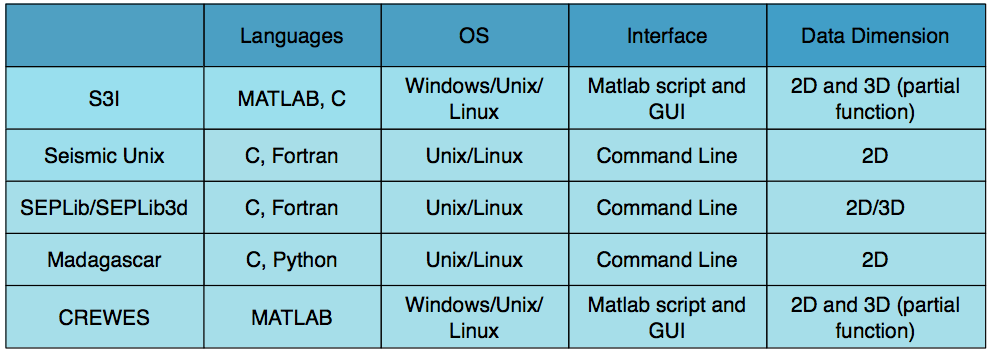
\includegraphics[scale=.42]{figures/open_package_list.png}
\caption{Comparison of open source packages\cite{CeGPS3I}}
\label{open_package_list}
\end{figure}

\section{Handle the Big Data}
Actually, all open source seismic softwares discussed in previous section are only used in research area. Not to say performance of MATLAB codes, all of these packages are sequential codes that could not run in parallel, so it is impossible for a company using such softwares in commerial purpose. As discussed in privious charpter, even the popular used HPC technology could not handle big data problems. 

Big data distinguish itself from traditional data in three main characteristics: volume, variety and velocity\cite{CharactOfBigData}. The increasing of volume size make it impossible to store and process data in single node, which is a big challenge to existing storage solution and computation model. Variety means data may come from different sources with different types, so the available RDBMS could not handle it, and how to store data efficiently and how to retrieve useful data for analysis are main problems to solve. As for the high velocity, which means large data are generated in real time environment and need to be analyzed on time due to the lifetime of data utility\cite{CharactOfBigData}, it also involves data storage and processing model issues. Through research and pratice in last decade, there are already several common open platforms that could handle big data effectively. In \cite{ChallengeOfBigData}, the author groups big data technologies into two categories, big data processing and big data persistence. Basing on data source and timeliness requirement, there are three main data processing platforms: batching processing, streaming processing and fast\/real-time processing. Distributed file system that could handle big data and NoSQL(Not Only SQL) that focus on unstructured data are main solutions in big data persistence, and the target of them are provide both high-availability and scalability to processing application.  

\subsection{Batch Processing Platform}
Google first released two papers on GFS(Google File System) in \cite{GhemawatGFS945450} and MapReduce in \cite{DeanMSD1251264} at 2004, which had been used by Google for storing and analyzing web search data. Basing on such ideas, Apache proposed open source implementation named Hadoop \cite{ApacheHadoop}. Hadoop provides big data storage solution with HDFS and big data processing modle with MapReduce. There are a lot of software packages built on Haoop, such as HBase \cite{ApacheHBase}, Hive \cite{ApacheHive} and Pig \cite{ApachePig} etc., which make Hadoop become the most popular ecosystem on big data batch processing. In \cite{2432874MohammadzaheriDISRAYMapReduce}, \cite{6118958RizvandiMapRecudePKTM} and \cite{2745578AddairSeismicSignalHadoop}, some traditional signal processing and migration algorithms are already implemented on MapReduce platform. \cite{6427595WangMultimediaMapReduce} built a large scale multimedia data mining platform by using MapReduce framework, where the processing dataset is similar to seismic image. However,  MapReduce only supports batch processing and relies on HDFS for data distribution and synchronization, which have significant overheads for iterative algorithms. Furthermore, there is no support for streaming and interactive processing in MapReduce, which becomes the biggest hole for supporting time sensitive data processing applications.

\subsection{Streaming Processing Platform}
Storm \cite{ApacheStorm} originally conceived and built by the team at Twitter to analyze the tweet stream in real time. The goal of Storm is to make it easy to write and scale complex real time computations on a cluster of computers. Storm guarantees that every message will be processed, and it is able to process millions of tweet messages per second with a small cluster. 
Storm YARN enables Storm applications to utilize the computational resources in a Hadoop cluster along with accessing Hadoop storage resources such as HBase\cite{ApacheHBase} and HDFS. Although it is scalable to process streaming messages, Storm is not designed for batch and interactive execution, and mostly focuses on text based message processing. 

\subsection{In-Memory Hybrid Platform}
To reduce the overhead of shuffling data into HDFS and to support more widely used iterative algorithms, there raised several in-memory computing frameworks. Apache Flink \cite{ApacheFlink} is a fast and reliable large-scale data processing engine, which is originally coming from Stratosphere \cite{Alexandrov2013Stratosphere}. It provides in-memory data sets, query language, machine learning algorithms and interfaces handling streaming data. Besides providing batch processing function, Flink is good at incremental iterations by pipelining data in an execution engine, which makes it suitable for most machine learning algorithms. 
Spark \cite{ZahariaSCC1863113} is a quick-rising star in big data processing systems, which combines the batch, interactive and streaming~\cite{ZahariaDSE2342773} processing models into a single computing engine. It provides a highly scalable, memory-efficient, in-memory computing, real-time streaming-capable big data processing engine for high-volume, high-velocity and high-variety data. Moreover, it supports high-level language Scala that combines both object-oriented programming and functional programming into a single programming model. The innovative designed Resilient Distributed Dataset (RDD)~\cite{SparkRDD} and its parallel operations provide a scalable and extensible internal data structure to enable in-memory computing and fault tolerance. There is a very active, and fast-growing research and industry community that builds their big data analytics projects on top of Spark. 
Apache Ignite \cite{ApacheIgnite} In-Memory Data Fabric is a high-performance, integrated and distributed in-memory platform for computing and transacting on large-scale data sets in real-time, orders of magnitude faster than possible with traditional disk- or flash-based technologies. 
However, all these frameworks are built for general propose cases and are focused on data parallelism with improved MapReduce model, and there is no communication mechanism between workers, which does not fit to some iterative seismic algorithms requiring frequent data communication among workers. The global memory technique could be achieved by adding communication layers to existing platforms or by storing data into database. 

\section{Big Data Persistence and Data Locality}
With the growing exponentially of the seismic data volumes, how to store and manage the seismic data becomes a very challenge problem. The legacy HPC computing model needs to distribute data to every worker node, which will consume more time on data transferring. The trend toward big data is leading to transitions in the computing paradigm, and in particular to the notion of moving computation to data, also called near-data-processing(NDP) \cite{6871738BalasubramonianNDP}. In Data Parallel System such MapRecuce \cite{6217449GuoDataLocalityMapReduce}, clusters are built with commodity hardware and each node takes the roles of both computation and storage, which makes it possible to bring computation to data. In \cite{6267846PerroneReducingDataMovement}, it presented an optimized implementation of RTM by experiments with different data partitioning, keeping data locality, and reducing data movement. In \cite{NextDataCenterVisualization}, it proposed a remote visualization solution by introducing GPU computing into cluster, which could overcome problems of dataset size by reducing data movements to local desktop. In \cite{6092321VoParaVisMapReduce}, it evaluated the suitability of MapReduce framework to implement large-scale visualization techniques by combining data manipulation and data visualization system on cluster. 

Besides  binary seismic data, there are huge amount semi-structured data and metadata generated at seismic data acquisition and processing. There are some obvious limitations of traditional RDBMS to handle this kind of big data; RDBMS is not flexible to handle different types of data, and there are also scalability and performance limitations on RDBMS. The NoSQL database is designed to be more suitable in such a scenario. HBase \cite{ApacheHBase} is a distributed, scalable and column\-based database after Google's Bigtable \cite{BigTableChang1365816} which is good at random, realtime read/write access to big data. Cassandra \cite{ApacheCassandra} is a distributed NoSQL database designed to handle large amount of data that could achieve linear scalability and fault-tolerant ability without compromising performance. MongoDB \cite{MongoDBNoSQL} is a document-oriented NoSQL database that casts focus on flexible data model and highly scalability. Redis \cite{RedisNoSQL} is a data structure server that provides key-value cache and storage, and it works with in-memory dataset thus could achieve outstanding performance. Based on the characteristics of seismic data, Cassandra could be used to save metadata and provide dataset to Spark, while Redis could be used to store intermediate data shared by all workers.Inspired by Google’s Dremel, Apache Drill \cite{ApacheDrillMain} is a low latency distributed query engine for large-scale datasets, including structured and semi\-structured/nested data. 

\section{New Algorithms\&Models Applied on Seismic Data}
With the increasing volume size of seismic data, the algorithms applied on data also become more sophisticated to extract valuable information. Some advanced machine learning algorithms are already used in this area. \cite{7067356ChakiPredictSandNeuralNetwork} used artificial neural network (ANN) to predict sand fraction from learning multiple seismic attributes such as seismic impedance, amplitude, and frequency. In \cite{6234749DengSVMPredictReservoir}, it set up a model by feeding five seismic attributes and the reservoir thickness to train Support Vector Machines (SVM) and then used it to predict the reservoir thickness. \cite{4026836MachadoNerualNetworksFault} used meta-attributes to train multi-layer neural networks and evaluated the effectiveness of the new generated seismic fault attribute. \cite{6707117KaurPWaveANN} used Back Propagation Neural Network (BPNN) for the automatic detection and identification of local and regional seismic P-Waves. 
Petuum \cite{Dai2013Petuum} is distributed machine learning framework that is focused on running generic machine learning algorithms on big data sets and simplifying the distributed implementation of programs. Based on characteristics of machine learning algorithms, Petuum provides iterative-convergent solutions that quickly minimize the loss function in a large-scale distributed cluster. Since these frameworks such as Petuum and Graphlab \cite{DatoGraphLab} are designed specially for machine learning algorithms, they could get better performance comparing with other general purpose MapReduce frameworks that emphasize on consistency, reliability and fault tolerance. 

In summary, traditional open source seismic package clould only handle small volume size seismic data, and although there are already many research projects trying to solve the big data problem, but there is still no perfect solution designed specific to seismic data. The MapReduce platform and its predecessors are too common to support complicate seismic algorithms, while some other platforms either emphasize on performance of computation or model optimization in narrow specific area. All existing opensource seismic packages are not friendly for domain-specific experts.
To make it easy for geophysicists and data scientists processing and analyzing big seismic data, a new platform is needed by incorporating the advances of big data research into the industry. Such a platform should not only be capable of processing big data efficiently and running advanced analytics algorithms, but also should achieve high usability, fault tolerance and good scalability. Data management and distribution supporting both structured and unstructured need to be hiden in order to allow geophysicists to utilize the platform easily. Moreover, typical seismic analytics algorithm templates and workflow would be very useful to simplify their work and to improve overall performance. 


%%%%%%%%%%%%%%%%%%%%%%%%%%%%%%%%%%%%%%%%%%%%%%%%%%%%%%%
%\subsection{Subsection}

%A table example is going to follow.

%\begin{table}[H]
%\centering
%\caption{This is a table template}
%\begin{tabular}{|l|c|c|c|c|c|}
%\hline
%Product & 1 & 2 & 3 & 4 & 5\\
%\hline
%Price & 124.- & 136.- & 85.- & 156.- & 23.-\\
%Guarantee [years] & 1 & 2 & - & 3 & 1\\
%Rating & 89\% & 84\% & 51\% & & 45\%\\
%\hline
%\hline
%Recommended & yes & yes & no & no & no\\
%\hline
%\end{tabular}
%\label{tab:template2}
%\end{table}
%\subsubsection{This is a subsubsection}


